%%%%%%%%%%%%%%%%%%%%%%%%%%%%%%%%%%%%%%%%%%%%%%%%%%%%%%%%%%%%%%%%%%%%
%% I, the copyright holder of this work, release this work into the
%% public domain. This applies worldwide. In some countries this may
%% not be legally possible; if so: I grant anyone the right to use
%% this work for any purpose, without any conditions, unless such
%% conditions are required by law.
%%%%%%%%%%%%%%%%%%%%%%%%%%%%%%%%%%%%%%%%%%%%%%%%%%%%%%%%%%%%%%%%%%%%

\documentclass[
  digital, %% This option enables the default options for the
           %% digital version of a document. Replace with `printed`
           %% to enable the default options for the printed version
           %% of a document.
  table,   %% Causes the coloring of tables. Replace with `notable`
           %% to restore plain tables.
  lof,     %% Prints the List of Figures. Replace with `nolof` to
           %% hide the List of Figures.
  lot,     %% Prints the List of Tables. Replace with `nolot` to
           %% hide the List of Tables.
  %% More options are listed in the user guide at
  %% <http://mirrors.ctan.org/macros/latex/contrib/fithesis/guide/mu/sci.pdf>.
  oneside,
]{fithesis3}
%% The following section sets up the locales used in the thesis.
\usepackage[resetfonts]{cmap} %% We need to load the T2A font encoding
\usepackage[T1,T2A]{fontenc}  %% to use the Cyrillic fonts with Russian texts.
\usepackage[
  main=czech,  %% By using `czech` or `english` as the main locale
                %% instead of `slovak`, you can typeset the thesis
                %% in either Czech or English, respectively.
  english, german, russian, czech, slovak %% The additional keys allow
]{babel}        %% foreign texts to be typeset as follows:
%%
%%   \begin{otherlanguage}{german}  ... \end{otherlanguage}
%%   \begin{otherlanguage}{russian} ... \end{otherlanguage}
%%   \begin{otherlanguage}{czech}   ... \end{otherlanguage}
%%   \begin{otherlanguage}{slovak}  ... \end{otherlanguage}
%%
%% For non-Latin scripts, it may be necessary to load additional
%% fonts:
\usepackage{paratype}
\def\textrussian#1{{\usefont{T2A}{PTSerif-TLF}{m}{rm}#1}}
%%
%% The following section sets up the metadata of the thesis.
\thesissetup{
    date            = \the\year/\the\month/\the\day,
    university      = mu,
    faculty         = sci,
    department      = Ústav chemie,
    departmentEn    = Department of Chemistry,
    extra = {
      departmentCs  = Department of Chemistry,
    },
    programme       = Fyzikální chemie,
    programmeEn     = Physical Chemistry,
    extra = {
      programmeCs   = Chemistry,
    },
    field           = Fyzikální chemie,
    fieldEn         = Physical Chemistry,
    extra = {
      fieldCs       = Physical Chemistry,
    },
    type            = mgr,
    author          = Petra Hrozková,
    gender          = f,
    advisor         = doc. Markéta Munzarová Dr. rer. nat. ,
    title           = Studium elektronové struktury fosfosilikátů a jejich silikátových          prekurzorů metodou DFT,
    TeXtitle        = A DFT study of the Electronic Structure of Silicate Precursors for Phosphosilicates
.
,
    titleEn         = A DFT study of the Electronic Structure of Silicate Precursors for Phosphosilicates
,
    TeXtitleEn      = A DFT study of the Electronic Structure of Silicate Precursors for Phosphosilicates
,
    extra = {
      titleCs       =A DFT study of the Electronic Structure of Silicate Precursors for Phosphosilicates
,
      TeXtitleCs    = A DFT study of the Electronic Structure of Silicate Precursors for Phosphosilicates
,
    },
    keywords        = {kľúčové slovo 1, kľúčové slovo 2, ...},
    TeXkeywords     = {kľúčové slovo 1, kľúčové slovo 2, \ldots},
    keywordsEn      = {keyword1, keyword2, ...},
    TeXkeywordsEn   = {keyword1, keyword2, \ldots},
    extra = {
      keywordsCs    = {klíčové slovo 1, klíčové slovo 2, ...},
      TeXkeywordsCs = {klíčové slovo 1, klíčové slovo 2, \ldots},
    },
    abstract      = {This is the abstract of my thesis, which can

                     span multiple paragraphs.},
    abstractEn    = {This is the English abstract of my thesis, which can

                     span multiple paragraphs.},
    extra = {
      abstractCs   = {This is the Czech abstract of my thesis, which can

                      span multiple paragraphs.},
    },
    thanks        = {These are the acknowledgements for my thesis, which can

                     span multiple paragraphs.},
    bib           = example.bib,
    %% Uncomment the following line (by removing the % symbol at
    %% the beginning) and replace `assignment.pdf` with the
    %% filename of your scanned thesis assignment.
    % assignment    = assignment.pdf,
}
\usepackage{makeidx}      %% The `makeidx` package contains
\makeindex                %% helper commands for index typesetting.
%% These additional packages are used within the document:
\usepackage{paralist} %% Compact list environments
\usepackage{amsmath}  %% Mathematics
\usepackage{amsthm}
\usepackage{amsfonts}
\usepackage{url}      %% Hyperlinks
\usepackage{mhchem}
\usepackage{chemfig}
\usepackage{subfigure}
\usepackage{listings} %% Source code highlighting
\usepackage{braket}
\usepackage{tikz}
\DeclareUnicodeCharacter{2009}{ }% support older LaTeX versions
\DeclareUnicodeCharacter{2212}{ }% support older LaTeX versions


%\renewcommand{\baselinestretch}{1.2}
%\usepackage{chemmacros}

\lstset{
  basicstyle      = \ttfamily,%
  identifierstyle = \color{black},%
  keywordstyle    = \color{blue},%
  keywordstyle    = {[2]\color{cyan}},%
  keywordstyle    = {[3]\color{olive}},%
  stringstyle     = \color{teal},%
  commentstyle    = \itshape\color{magenta}}
\usepackage{floatrow} %% Putting captions above tables
\floatsetup[table]{capposition=top}
\begin{document}


\chapter{Úvod}
 Tato práce vznikla za podpory projektů CERIT Scientific Cloud (LM2015085) a CESNET (LM2015042) financovaných z programu MŠMT Projekty velkých infrastruktur pro VaVaI.

\section{Experimentální motivace}
Cílem této práce je podat vysvětlení některých experimentálních jevů, které byly pozorovány u silikofosfátových polymerů. Studium vysoce porézních silikofosfátů je jedním ze zaměření skupiny anorganické a~materiálové chemie na našem ústavu. Studie prezentované v této práci se zaměřuje na na přítomnost hypervalentního, tj. pěti nebo šestikoordinovaného křemíku, v jednotlivých strukturách. Obecný pohled na hypervalency poskytuje Rundleovo a Piementelovo schéma, kde se objevují elektronově-bohaté tří-centerní vazby \cite{405827} \cite{Munzarova2001}. \\
Amorfní struktura silikofosfátových xerogelů však neumožňuje jejich přímou strukturní charakterizaci. Důležitou součástí práce bylo navržení vhodných strukturních modelů. Modely navržené v této práci byly motivovány rentgenovými struktruami analogických periodických struktur \cite{C3NJ00721A} \cite{C4TA06823H} anebo příbuznými strukturami, které budou dále popsány. Dále byla využita data z NMR spektroskopie, z nichž byly odvozeny informace o výši koordinace křemíku a složení ligandů(fosfátové vs. organické estery) \cite{Styskalik2015thesis}. Druhou součástí práce byl podrobnější pohled na chemickou vazbu ve zvolenných modelech silikofosfátových polymerů. Pro analýzu chemické vazby byla použita teorie přirozených orbitalů a Mullikenova populační analýza.


\section{Silikofosfátové polymery}
Nejčastější formou výskytu křemíku v přírodě jsou křemičitany, sloučeniny obsahující křemík tetraedricky koordinovaný čtyřmi atomy kyslíku. Existují však i minerály s vyšší koordinací, např. thaumasit \cite{Edge:a08100}. Vzhledem k vysokému významu křemíku v přírodě jsou křemičitany rozsáhle připravovány a studovány i laboratorně. Oxid křemičitý \ce{SiO2} je po vodě nejvíce studovanou sloučeninou. Díky tomu, že \ce{Si^4+} je velikostně snadno zaměnitelný za \ce{Al^3+} nebo \ce{P^5+}, vznikají pak hlinitokřemičitany, obsahující Si-O-Al (zeolity), nebo fosfokřemičitany, obsahující Si-O-P, tj. silikofosfáty. Obě skupiny sloučenin jsou rozsáhle studovány. Konkrétně silikofosfátové polymery mají zajímavé fyzikální a chemické vlastnosti. Příkladem je Brønstedovská kyselost nebo vysoká protonová vodivost. Několik z možných uplatnění silikofosfátových polymerů mohou být konduktory, elektrolyty, optická vlákna a biokompatibilní materiály.\\
Silikofosfáty i hlinitokřemičitany jsou charakteristické svojí trojrozměrnou  porézní strukturou. Naše pozornost je v této práci soustředěna na silikofosfáty. Předpokládaná struktura připravených silikofosfátů studovaných v předchozích experimentálních prací je znázorněna na obrázku \ref{si_polymer_cely} \cite{Styskalik2015thesis}. Charakteristickou vlastností struktur silikofosfátů je uspořádání jednotek Si-O-P do cyklů. \\
Ačkoliv nejnovější struktura zahrnuje dvanáctičlenové cykly vzniklé trojnásobným opakování motivu Si-O-P-O (Pinkas et. aln Inorganic Chemistry), struktury s hypervalentním křemíkem obsahují osmičlenné cykly vzniklé dvojnásobným opakování jednotky Si-O-P-O .
 \begin{figure}[h!]
 \caption{RTG struktura cyklu Si-O-P-O, \cite{C4TA06823H}.}
   \center
   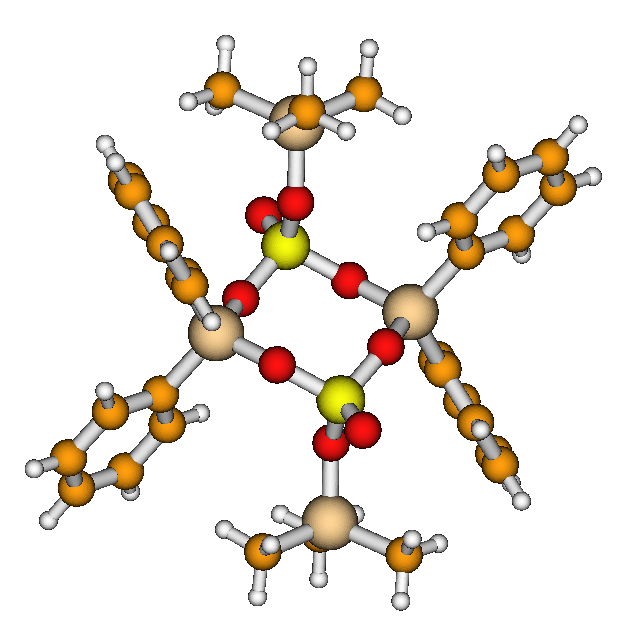
\includegraphics[width=10cm]{rtg_kruh_samostatne.png}
   \label{rtg_cyklus}
   \end{figure}
  Obrázek \ref{si_polymer_cely} znázorňuje předpokládanou strukturu silikofosfátového xerogleu se třemi druhy křemíkových center (koordinace čtyřmi fosfáty, šesti fosfáty, anebo čtyřmi fosfáty a dvěma organickými estery současně) a osmičlennými cykly Si-O-P.  Konkrétní podoba osmičlenného cyklu byla ověřena metodou RTG \cite{C4TA06823H}. Stupeň koordinace křemíku a~současně velikost pórů se ukázala být silně závislá na typu prekurzoru. Pokud byl ve výchozích sloučeninách jeden z fosfátů nahrazen methylovou skupinou přímo vázanou na křemík, ve výsledném xerogelu se nevyskytovaly oktaedricky koordinované křemíky a velikost pórů byla větší. Konkrétní podobu okolí křemíku je ukázáno ve schématu níže. Koordinační okolí bylo získáno kombinací NMR dat a IR dat \cite{C4TA06823H}.
  \begin{center}
  \begin{tikzpicture}[thick,scale=0.6, every node/.style={scale=0.6}]
  \node at (-4,1) { \chemfig{
                  HO% 2
        -[:330,,2]P% 1
                     (
           -[:270,,,1]OH% 4
                     )
                     (
                =[:30]O% 5
                     )
       -[:210,,,2]HO% 3
    }};
    \node at (-2,3){\chemfig{
                   R% 2
            -[:270]Si% 1
                      (
                     <:O% 4
                -[,,,1]P% 7
                      )
                      (
                <[:300]O% 5
            -[:270,,,1]P% 6
                      )
            -[:210]O% 3
        -[:150,,,1]P% 8
    }};
  \node at (4,1.5)  {\small \chemfig{
                  HO% 2
        -[:330,,2]P% 1
                     (
           -[:270,,,1]OH% 4
                     )
                     (
                =[:30]O% 5
                     )
       -[:210,,,2]HO% 3 \schemestop
    }};
  \node at (6,3)  {\chemfig{
                   R% 2
            -[:270]Si% 1 \schemestop
                      (
                     <:O% 4
                -[,,,1]P% 7
                      )
                      (
                <[:300]O% 5
            -[:270,,,1]P% 6
                      )
            -[:210]O% 3
        -[:150,,,1]P% 8
    }};
  \node at (9,1.5) { \chemfig{
              O% 2
       =[:330]P% 1
                 (
       -[:270,,,1]OH% 3
                 )
                 (
        -[:60,,,1]OH% 5
                 )
       -[,,,1]OH% 4
    }};
  \end{tikzpicture}
    \end{center}
  \begin{center}
    \begin{tikzpicture}[thick,scale=0.6, every node/.style={scale=0.6}]
    \node at (-4.5,1) { \chemfig{
           O% 2
    =[:210]P% 1
              (
        -[:210]O% 4
    -[:240,,,1]Si% 7
              )
              (
        -[:270]O% 5
    -[:330,,,1]Si% 8
              )
    -[:120]O% 3
    -[:150]R% 6
}};
    \node at (-2,3){\chemfig{
               O% 2
     -[:270,,1]Si% 1
                  (
        -[:180,,,1]O% 3
                  )
                  (
      <:[:30,,,1]O% 5
                )
                  (
            -[,,,1]O% 5
                  )
    -[:270,,,1]O% 4
}};
    \node at (4,1.5)  {\chemfig{
           O% 2
    =[:210]P% 1
              (
        -[:210]O% 4
    -[:240,,,1]Si% 7
              )
              (
        -[:270]O% 5
    -[:330,,,1]Si% 8
              )
    -[:120]O% 3
    -[:150]R% 6
}};
    \node at (6,3) {\chemfig{
               O% 2
     -[:270,,1]Si% 1
                  (
        -[:180,,,1]O% 3
                  )
                  (
      <:[:30,,,1]O% 5
                )
                  (
            -[,,,1]O% 5
                  )
    -[:270,,,1]O% 4
}};
    \end{tikzpicture}
    \end{center}
   \cite{Styskalik2015thesis}.Silikofosfátové cykly jsou pak dále organizovány do vyšší stuktury skeletu mikroporézního (šířka pórů doo 2 nm) až mezoporézního (šířka póru 2-50 nm). Potvrzená struktura šestikoordinovaného křemíku je uvedena obrázku. Struktura byla získána metodou rentgenové difrakce \ref{rtg_koordinace_sest} \cite{C3NJ00721A}.

    Konkrétní metody příprav slikofosfátových sloučenin jsou uvedeny například v práci Aleše Stýskalíka. \\

\begin{figure}[h!]
\caption{Silikofosfátová síť, \cite{Styskalik2015thesis}. }
  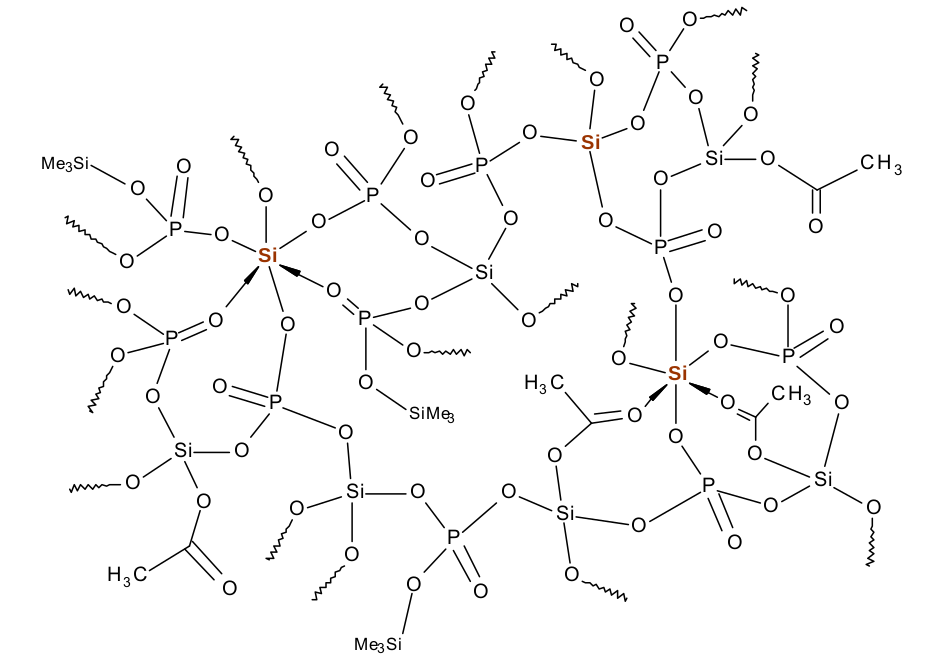
\includegraphics[width=12cm]{si_polymer_cely.png}
  \label{si_polymer_cely}
  \end{figure}

  \begin{figure}[h!]
  \caption{Struktura silikofosfátu získaná z RTG,\cite{C4TA06823H}. }
    \center
    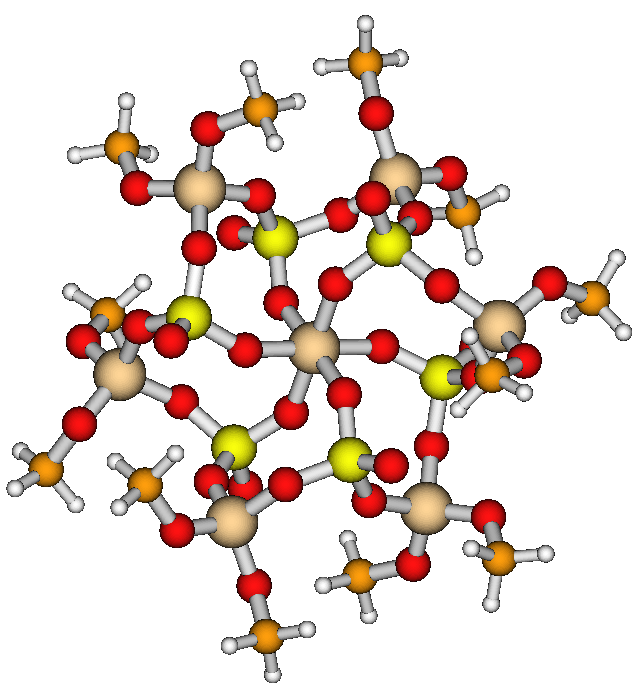
\includegraphics[width=10cm]{struktura_puvodni.png}
    \label{rtg_koordinace_sest}
    \end{figure}

\section{Hypervalence p-prvků}
První kvantitativní popis chemické vazby zavedl Lewis v roce 1916, kdy vazbu považoval za sdílení elektronového páru mezi dvěma atomy. Cílem párování bylo zaplnění valenčí vrsty a dosažení konfigurace vzácného plynu, tvz. oktetové pravidlo. Pro vodík platí dubletové pravidlo, Pravidlo elektronového oktetu říká, že  prvky $p$ skupiny chtějí mít ve své valenční vrstvě právě osm elektronů. Toho lze docílit vytvořením chemické vazby, excitací, nebo ionizací. Spárované elektrony, které se neúčastní vazby, se nazývají volné elektronové páry. Přísná lokalizace elektronů s pomocé vazebných orbitlaů v Lewisovské teorii ovšem nesouhlasila s pozorování pro organické sloučeniny s uhlíkem. Vysvětlení podal L. Pauling pomocí teorie valenčních vazeb a teorii hybridizace \cite{Munzarova1996thesis}.\\

Podle klasické teorie valenční vazby mohou $p$ prvky tvořit čtyři vazby. Z experimentálních pozorování je ale známo, že prvky $p$  tvoří i více než je číslo jejich atomových orbitalů, obvykle pět nebo šest. Příkladem můhou být sloučeniny xenonu, například \ce{XeF6}.
Sloučeniny, kde se vyskytuje jeden nebo více atomů s více než osmi elektrony (oktet) se nazývají hypervalentní/hyperkoordinované. Konkrétně křemík může vytvářet 4-,5- a 6- koordinované sloučeniny a stát se hypervalentní. Pro vysvětlení hypervalence p-prvků lze použít teorii hybridizace. Obecně se čtykoordinované sloučeniny vyskytují jako tetraedry, hybridizace $sp^3$. Pětikoordinované sloučeniny tvoří trigonální bipyramidu, hybridizace $sp^3d$. A šestikoordinované sloučeniny tvoří oktaedr, hybridizace $sp^3d^2$.\\

Čtyřkoordinovaný křemík splňuje tetraedrické uspořádání. Při zvýšení koordinace na pět by měla být pozorována trigonální bipyramida, $sp^3d$. Výskyt $d$ orbitalu ve vazbě ale způsobuje nárust energie vazby na více než 200 kcal/mol. Z tohoto důvodu se předpokládá, že $d$ orbitaly se podílejí pouze na polarizaci porbitalů. Pentavalentní koordinace by měla být realizována jako $3sp^2$ hybridizace doplněna třícenterní, čtyřelektronovou vazbou $3c-4e$ s p orbitalem. V pětikoordinovaných sloučeninách se ale spíše uvažuje hybridizace $sp^2$ a jedna vazba $3c-4e$ s $p$ orbitalem, právě kvůli energii $d$ orbitalů.\\
Hypervalentní sloučeniny jsou lepší Lewisovské kyseliny díky $d+$ efektu na centralním křemíku. Důvodem je přesun elektronové hustoty na ligandy skrz nevazebné MO a podpora $3c-4e$ vazby. Rozložení elektronové hustoty molekulu stabilizuje a z tohoto důvodu se v hypervalentních sloučeninách vyskytují jako ligandy prvky s vysokou elektronegativitou. Tento jev dobře popisuje tzv. Bentovo pravidlo:"Elektronegativní prvek dáva přednost vazbe s větším p-charakterem."\cite{hypervalentsiliconmacmillangroup2005}.\\
Pro křemík v koordinaci šest lze také předpokládat, že význam $d$ orbitalů nebude významný vzhledem k jejich energii. I zde se do vazby zapojí $3c-4e$ vazby\cite{Wagler2014}.\\
Další možnost interpretace hypervalence je založena na vysoké iontovosti vazby na křemíku. Obecně iontovost s koordinačním číslem roste.
Navíc chování vazby Si-ligand silně závisí na samotném ligandu a sterickém a elektronovém uspořádání. Hovoříme o Lewisovské kyselosti křemíkové vazby s elektronegativním atomem. Chování křemíku lze rozdělit na iontové, sigma vazebné a donor interakci \cite{Wagler2014}.\\


\section{Hypervalence sloučenin křemíku}\label{teorie_hypervalence}
V případě čtyřkoordinovaných sloučenin křemík poskytuje do vazeb všechny své valenční elektorny. Ve vyšším koordinačním stupeni už může křemík poskytnou pouze prázdné orbitaly a proto chová se jako Lewisovská kyselina. Obecně mají Lewisovské kyseliny prázdné molekulové orbitaly, které leži dostatečně blízko obsazeným MO \footnote{MO = Molekulový orbital} konjugované báze.

Z experimentu je známo, že \ce{SiO4} je dostatečnou Lewisovskou kyselinou, aby křemík mohl přímo reagovat s Lewivoskou bazí. Pokud je jeden z kyslíku ve struktuře nahrazen uhlíkem, schopnost navyšovat koordinaci je ztracena. Stejný jev pozoroval Aleš Sýskalík a spol. \cite{Styskalik2015thesis} a to vedlo k hypotéze o snížení Lewisovské kyselosti křemíku při tvorbě přímé vazby Si-C. Naopak pětikoordinovaný křemík je lepší Lewisovskou kyselinou než čtyřkoordinovaný a hypervalency podporuje. Atomy jako uhlík, dusík, kyslík, fluor nebo chlor podporují navyšování koordinace křemíku \cite{Wagler2014}.\\
Existující, experimentálně připravené hypervalentní sloučeniny s křemíkem lze rozdělit podle jednotlivých ligandů a jejich poloze v periodické tabulce. Křemík je schopen tvořit hypervalentní sloučeniny s fluorem, příkladem může být struktura  \ce{(SiF6)^{2-}} \ref{si_f6} \cite{memoriesphysiquelussac}. Tato struktura byla připravena v 19. století a považuje se za první připravenou sloučeninu křemíku v koordinaci šest. Pokud budeme postupovat ve skupine halogenů dolů, dalším ligandem by měl být logicky chlor. Sloučenina \ce{SiCl6^{2-}} není známá, naopak \ce{GeCl6^{2-}} ano. Schopnost atomu tvořit hypervalentní sloučeniny roste ve skupině dolů. Germanium má tedy vysokou schopnost tvořit hypervalentní sloučeniny. Oproti tomu křemík potřebuje ligand s výrazně vyšší elektronegativitou. Hypervalentní sloučeniny s chlorem byly proto připraveny až později, například \ref{si_cl_o} \cite{LAZAREV199716}.\\
Ve sloučeninách s křemíkem může být fluor nahrazen dalšími $p$ prvky, například kyslíkem \ref{si_o_f} \cite{C0DT01115K} nebo kyslíkem a vodíkem \ref{si_fluor_vodik_kyslik} \cite{BOYER19812165}.
Jako ligand společně s fluorem může být použit i dusík \ref{si_f_n}  \cite{C0DT01115K} nebo uhlík \ref{si_with_fluor_carbons} \cite{kremikfluorcarbon}.\\
Schopnost křemíku navyšovat koordinaci existuje i ve sloučeninách s kyslíkem \ref{si_only_o} \cite{flyn1969}. Strukutra \ce{Sio6} se vyskytuje také v přírodě v minerálu thaumasite \cite{Edge:a08100}. Kyslík může být nahrazen dusíkem  \ref{si_o_n} \cite{Wagler2014} nebo uhlíkem a dusíkem  \ref{si_n_o_c} \cite{Wagler2014}\\
Je zajímavostí, že existují i sloučeniny pouze s vazbou křemík-uhlík \ref{si_only_c} \cite{A901953G}\cite{Wagler2014}.
 \begin{figure}
 \begin{center}
   \subfigure[]{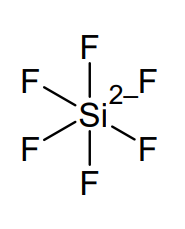
\includegraphics[width=2cm]{si_f6.png}\label{si_f6}}
 \subfigure[]{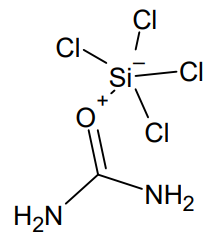
\includegraphics[width=3cm]{si_cl_o.png}\label{si_cl_o}}
 \subfigure[]{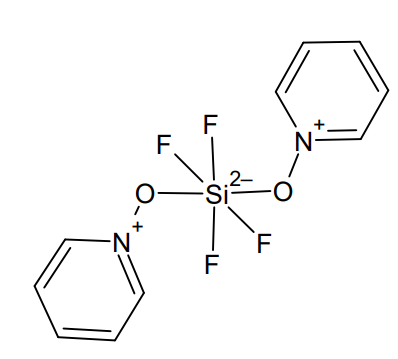
\includegraphics[width=5cm]{si_o_f.png}\label{si_o_f}}
 \subfigure[]{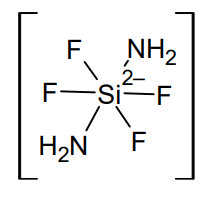
\includegraphics[width=3cm]{si_f_n.png}\label{si_f_n}}
 \subfigure[]{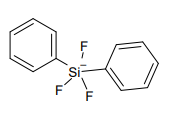
\includegraphics[width=5cm]{si_with_fluor_carbons.png} \label{si_with_fluor_carbons}}
 \subfigure[]{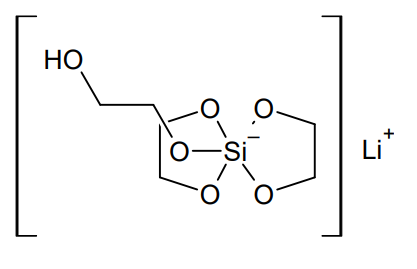
\includegraphics[width=5cm]{si_only_o.png} \label{si_only_o}}
 \subfigure[]{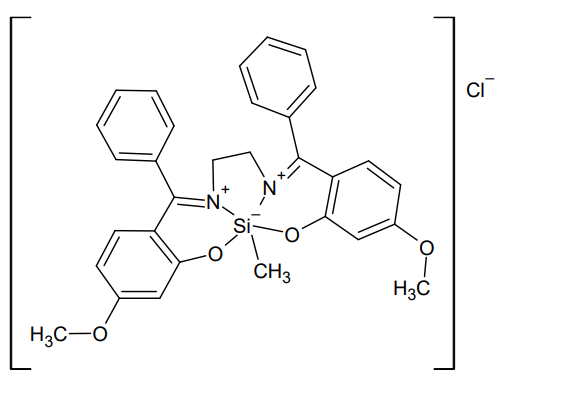
\includegraphics[width=5cm]{si_n_o_c.png}\label{si_n_o_c}}
 \subfigure[]{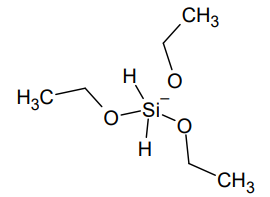
\includegraphics[width=5cm]{si_fluor_vodik_kyslik.png} \label{si_fluor_vodik_kyslik}}
 \subfigure[]{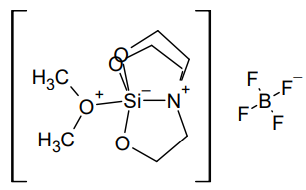
\includegraphics[width=5cm]{si_o_n.png} \label{si_o_n}}
 \subfigure[]{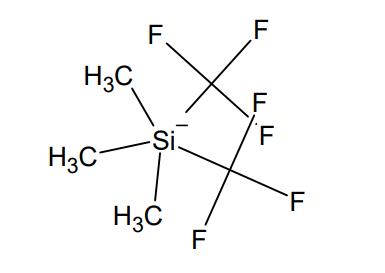
\includegraphics[width=5cm]{si_only_c.png} \label{si_only_c}}
 \label{shrnuti_struktury_kremik}
 \end{center}
 \end{figure}

\section{Formulace teoretického problému}
Postupně jsme hlavní otázku, řešenou v této práci, zformulovali do následující podoby: Jaká je souvislost mezi kombinací ligandů na čtyřkoordinovaném Si a Lewisovskou kyselostí těchto čtyřkoordinovaných sloučenin, vedoucí ke sklonu křemíku zvýšit svoji koordinaci na pět nebo šest ligandů.
Z tohoto důvod jsme se rozhodli porovnávat Lewivoskou kyselost, abychom určili stabilitu jednotlivých částí silikofosfátů. Navíc jsme se snažili najít parametr, který by umožnil určit velikost póru v závislosti na okolí křemíku. Pro tuto práci jsem zvolila tři úrovně zkoumání silikofosfátů, rozdělené podle velikosti modelů. Velké modely sloužily jako odhad skutečné struktury silikofosfátů, včetně jednotlivých pórů. Středně velké modely byly stále dost komplexni, ale již umožňovaly podroběnjší pohled na chemickou vazbu Si-C. Malé modely byly snadné pro porozumění. \\
Jako prostředek ke zkoumání silikofosfátů jsem zvolila molekulové orbitaly, které poskytují široké spektrum informací o molekule, vazbách, struktuře, kyselosti,\dots  Analýza byla provedena s pomocí teorie funkcionální hustoty(DFT)\footnote{DFT - Density Functional Theory, česky Teorie funkcionálu hustoty}, která se řadí mezi kvatově-chemické metody. Pro porovnání byla stejná analýza udělána s pomocí teorie Přirozených molekulových orbitalů(NBO)\footnote{NBO - Natural Bond Orbitals, česky Přirozené Molekulové orbitaly}. Výhoda přístupu NBO je snadnější převod čísel do chemického významu. Pro určení Lewisovské kyslelosti bylo stěžejní určení procenta $s$ a $p$ orbitalů křemíku v antivazebných orbitalech.  V NBO analýze jsme určovali procento vazebných orbitalů (BD) ligandu. V MPA analýze jsme určovali procento $s$ a $p$ orbitalů křemíku a ligandech.
\newpage
\chapter{Metody kvantové chemie}
Chování elektornů v molekulách však nelze popsat rovnicemi ani jazykem klasické mechaniky. Elektrony totiži vykazují typické kvantově-mechanické chování, projevují se diskrétním spektrem energií, vlnovým chováním ve smyslu difrakce nebo např. fotoelektrického jevu. Nelze je proto charakterizovat jejich jednotlivými polohami a hybnostmí, jediný přijatelný popis lze udělat pomocí tzv. vlnové funkce.
\section{Kvantově-mechanický popis elektronové struktury}
Současné chápání struktury , reaktivity a spektroskopického chování ůátek je založeno na detailní znalosti rozložení a energií elektronů v atomech a molekulách. Vlnová funkce se zpravidla označuje řeckým písmene $\Psi$ a je řešením Schrödingerovy vlnové rovnice \ref{schr_rce}. Levá strana Schrodintrovy rovnice vyjadřuje působení tzv. Hamiltoniánu ($\widehat{H}$) neboli operátoru energie na vlnovou funkci $\Psi$. Pravá strana Schrödingerovy rovnice vyjadřuje fakt, že lze nalézt takové vlnové funkce $\Psi$, které se působením $\widehat{H}$ pouze vynásobí konstantou $E$, která má význam energie. Řešením Schrödingerovy rovnice jsou tedy jednak možné hodnoty energie elektronů sytemů a jednak samotná vlnová funkce $\Psi$, která v sobě dle tzv. Bornovy interpretace obsahuje informaci o rozložení pravděpodobnosti vsýktytu elektronů v prostoru.
\begin{equation}
\hbar \Psi = E \Psi
\label{schr_rce}
\end{equation}
Analytické řešení Schrödingerovy rovnice josu dostupná pouze pro velmi malý okruh jednoduchých modelových Hamiltoniánů, jejiž nejdůležitější reprezentaty jsou kvantově chemický oscilátor, částice v jámě, atom vodíku a kation \ce{H2^{+}}. Dokonce ani pro atomu helia, který obsahuje pouze o jeden elektron více než atom vodíku, není dostupné plně analytické řešení Schringgerovy rovnice.
Z tohoto důvodu je v fyzikálních i chemických aplikacích nutno použít zjednodušení. Základní aproximací, kterou je třeba aplikovat pro všechny molekuly(včetně zmiňovaného iontu \ce{H2^{+}}, pro nejž lze vlnovou funkci elektronu vyjádřit analyticky) je tzv. Born-Oppenheimerova aproximace (B-O) \ref{B_O_approximace}. Její podstatou je oddělení pohybu elektronů od pohybu jader a lze ji dobře vysvětlit na základě termodynamické analogie vratného děje. Je-li například expanze plynu proti vnějšímu tlaku prováděna vratně, pohybuje se píst ve válci tak pomalu, že plyn je stále v rovnováze s okolím. Jeho tlak pak závisí pouze na pozici pístu. Podobně se jádra pohybují vzhledem k elektronům tak pomalu, že elektrony zaujmou pro každé rozmístění jader okamžitě nejvýhodnější rozložení. Proto můžeme energii elektronů považovat za závislou pouze na polohách jader. V rámci B-O aproximace lze tedy vlnovou funkci zapsat ve tvaru rovnice \ref{B_O_approximace}. $R_{\alpha}$ a $r_i$ jsou souřadnice elektronů. $R_{\alpha}$ souřadnice jader, $\Psi_{el}(r_i,R_{\alpha})$ je elektornová vlnová funkce, zavisející explicitně na polohách elektronů a parametricky na polohách jader, $\Psi_N(R_{\alpha})$ je jaderná vlnová funkce závislá pouze na polohách jader. $ \Psi_N(r_i, R_{\alpha}) $ je celková vlnová funkce \cite{lechamolecularmodeling}.
Vlnová funkce elektronů je řešením Schrongerovy rovnice, jež v operátoru energue zahrnuje pro každý elektron jeho kinetickou energii, přitahování jádry a jeho odpuzování se všemi ostatními elektrony. Posledně jmenovaný člen řídí pohyb každého elektronnu závisejícím na pohybu všech ostatních elektronů. V důsledků toho není elektronová Schrödingerova rovnice analyticky řešitelná.
Druhou základní aproximací kvantové chemie je přístup, v němž se okamžitá repulze jednoho elektornu s druhým nahrazuje repulzí prvního elektornu v časově rozmazanou distribucí druhého elektronu. Cílem je pak nalézt takové vlnové funkce obou (a všech dalších) jednotlivých elektronů, aby pro jeden elektron byla vlnová funkce tzv. orbital-optimální z hlediska minimalizace celkové energie. Tady například vlnová funkce pro elektron 1 musí být optimální mj. vzhledem k repulzím s elektronem 2 a obráceně, vlnová funkce pro elektro  2 musí být optimální mj. vzhledem k repulzím s elektronem 1. Celková vlnová funkce daného počtu elektronů, která se vyjadřuje jako tzv. Slaterův determinat z obsazených orbitalů, musí být z tohoto hlediska konzistentní sama se sebou, a proto se výše pospaná metoda nazývá Hartee-Fockova metoda selkonzistentního pole (HF-SCF). Vlnovou funkci lze zapsat jako Slaterův determinant, který zaručuje antisymetrii vlnové funkce vůči výměně polohových a spinových souřadnic. \ref{Slateruv_determinant}.
\begin{equation}
\psi =  \frac{1}{\sqrt{n!}}\begin{vmatrix}
\psi_1(1)\alpha(1) & \psi_1(1) \beta (1)  & \dots & \psi_{n/2}(1)\beta(1) \\
\psi_1(2)\alpha(2) & \psi_1(2) \beta (2) & \dots & \psi_{n/2}(2)\beta(2) \\
\vdots             & \vdots                           & \ddots & \vdots \\
\psi_1(n)\alpha(n) & \psi_1(n) \beta (n) & \dots & \psi_{n/2}(n)\beta(n)
\end{vmatrix}
\label{Slateruv_determinant}
\end{equation}
$\psi_i$ jsou prostorové části jednotlivých orbitalů, 1,2,\dots n jsou jednotlivé elektrony $i$, $\alpha(i)$ resp. $\beta(i)$ jsou spinové funkce těchto elektronů a $\frac{1}{\sqrt{n!}}$ je normovací konstanta.

Výsledná vlnová funkce se hledá následujícím způsobem: Na počátku výpočtu je zvolena určitá sada orbitalů, která jsou postupně jednotlivě optimalizována v poli elektronové hustoty zbylých orbitalů. Tím získáme novou sadu orbitalů, která se liší od původní sady orbitalů. Celý postup je opakován až do okmažiku, kdy mezi předchozí a následující sadou orbitalů rozdíly v energiích a elektronové hustotě klesnou pod předem zvolenou, dostatečně nízkou mez. Protože jsou výsledné energie vlastními funkcemi tzv. Fockova operátoru, který patří mezi tzv. Hermitovské operátory, jsou vypočítané orbitaly $\Psi_i$ a $\Psi_j$ příslušející různým vlastním hodnotám energie $\varepsilon $ a $\varepsilon_j$ orthogonální, tj. platí rovnice \ref{ortonormal_ortogonal}. Navíc lze zajistit, aby byly orthogonální každé dvě vlnové funkce příslušející stejné vlastní hodnotě energie $\varepsilon $, a také, aby každá vlnová funkce $\varphi_i$ tj. \ref{ortonormal_ortogonal}.
 \begin{equation}
 S_{ii} = \int \psi_i * \psi_i dx dy dz = 1 ~ \wedge ~ S_{ij} = \int \psi_i * \psi_j dx dy dz = 0
 \label{ortonormal_ortogonal}
 \end{equation}

\begin{equation}
  \Psi_{r_i,R_{\alpha}} = \Psi_{electronic}(r_i,R_{\alpha}) \cdot \Psi_{nuclear}(R_{\alpha})
  \label{B_O_approximace}
\end{equation}
Nejnižěí energie se hledá pomocí selfkonzistentní metody (viz. výše).
Nevýhoda HF-SCF přístupu je fakt, že neuvažuje korelaci elektronového pohybu, tj. fakt, že vybraný elektron nevnímá ostatní elektrony v jejich časově zprůměrovaném rozložení, nýbrž že vnímá okamžité polohy ostatních elektronů a přizpůsobuje jim svoji polohu. \\

Korelační energii lze vyjádřit jako rozdíl mezi přesnou nerelativistickou energii a HF limitou tzv. Hartree-Fockovou limitou, což je je energie Slaterova determinant, vyjádřeného v limitě nekonenčné báze. Ačkoliv korelační energie představuje méně než 1\% celkové tzv. energie elektronů, nemůže být zanedbána, pokud požadujeme chemickou přesnost tj. $1-2$ kcal/mol.
Korelační energii lze do výpočtu zahrnout tak, že výsledná vlnová funkce obsahuje mimo Slaterův determinant pro základnní stav také příspěvky Slaterových determinantů pro excitované stavy. Hovoříme pak o Post-Hartree-Fockových metodách. Mísením excitovaných determinantů lze započítat třemi základními způsoby. Předně jde o tzv. metodu konfigurační interakce (CI)\footnote{Configuration Interaction}, v níž jsou příspěvky excitací optimalizovány pomocí variační metody. Jiným možným způsobem započtení excitovaných determinantů je poruchová teorie zavedená M{\o}llerem a Plessetem. Poslední (a v reálné praxi nejpřesnější) metodou zahrnutí korelace pohybu elektronů prostřednictvím jejich excitaci do protivazebných MO je tzv. metoda spřažených klastrů. Její výhoda oproti CI je její správné škálování s velikostí systému díky tomu, že jednotlivými excitacemi zahrnuje i jejich superpozice.

 %#TODO poznámky k teoriím
\section{Teorie funkcionálu hustoty}
Systémy studované v této práci mají za cíl modelovat trojrozměrnou silikofosfátovou síť. Skládají se tedy ze silikátových a fosfátových jednotek. z nimž na každou připadá cca. 50 elektronů. Je proto velice důležité zvolit metodu, která bude spojovat vysokou přesnost s vysokou výpočetní efektivností. Současně je našim cílem porozumnění sklonu křemíku k hypervalenci, což indikuje pokud možno fyzikálně průzračnný jednoelektronový model. Všechny tyto požadavky splňuje Kohn-Shamova formulace metody funkcionálu hustoty\footnote{Z matematické analýzy je funkcionál operátor zobrazení z množiny funkcí do množiny obecně komplexních čísel.}\cite{bickelhaupt2007kohn}.\\
Základní myšlenka teorie funkcionálu hustoty pohlíží na systém elektronů a jader ze zcela jiného úhlu než tradiční $ab inito$ metody kvantové chemie, zahrnující metodu HF-SCF a její nadstavby. Posledně zmíněné metody zahajují popis molekuly od znalosti tzv. extermího potenciálu (nejčastěji daného polohami  a náboji jader) a pokračují přes kontrukci Hamiltoniánu, nalezení energií a vlnových funkcí až k výpočtu výsledné elektronové hustoty.\\
Základní teorémy metody funkcionálu hustoty (1. a 2. Hohensberg-Kohnův teorém) ukazují, že lze postupovat i opačně. Výsledná elektronová hustota zpětně jednoznačně určuje externí potenciál, a tedy i vlnovou funkci a všechny z ní odvozené měřitelné vlasnosti. Protože je elektronová hustota funkcí pouze tří souřadnic v prostoru (a nevztahuje se narozdíl od vlnové funkce k jednotlivým elektronům), lze metody funkcionálu hustoty využít k výpočtům, které jsou do výpočetní náročnosti srovnatelné s metodou HF-SCF, ale co do přenosti popisu metodu HF-SCF dalece převyšují.
\cite{jensen2007introduction}

Moderní DFT metody se začaly objevovat po roce 1964 jako výsledek Hohensberg-Kohnův teorémů. Aplikace v kvantově-chemických výpočtech se datují až od 90. let. Prvním Hohenberg-Kohn teorém (H-K) mluví o základním stavu. "Vnější potenciál  $V_ext$ je až na konstantu jednoznačným funkcionálem $\varrho(\vec{r})$, protože $V_ext$ určuje $\widehat{H}$, je úplný popis mnohačásticového základního stavu jednoznačným funkconálem $\varrho(\vec{r})$."\cite{PhysRev.136.B864} První H-K teorém můžeme schématicky vyjádřit takto:
\begin{equation}
\varrho_0 \Rightarrow {N, Z_A, R_A} \Rightarrow \widehat{H} \Rightarrow \Psi_0 \Rightarrow E_0
 \end{equation}
 Všechny vlastnosti základního stavu mnohaelektronového systému jsou tedy jednoznačně určeny elektronovou hustotou.

Samotná elektronová hustota je výsledkem druhého teorému. Ten říká, že nalezená elektornová hustota je jediná správná. Využívá variačního principu pro určení elektronové hustoty bez vlnové funkce. Správná elektronová hustota musí mít nejnižší energii a nejpřesnější energii.
\begin{equation}
E [\varrho_0] < E[\varrho ']
\end{equation}
 Energie excitovaného stavu musí být nižší než energie elektroové hustoty ostatních elektronů. Pro výpočetní chemii mají větší význam Kohn-Shamovy orbitaly, které byly výsledkem geniální myšlenky o rozdělení funkcionálu. Obecně je největší problém vyjádřit kinetickou energii elektornů. Ta se rozpadla na dvě části. Exaktní a korekční část.
\begin{equation}
E(\varrho(\vec{r})) = T_s[\varrho(\vec{r})] + J[\varrho(\vec{r})] + \int V_{EX}(\vec{r})\varrho(\vec{r})d\vec{r} + E_{XC}[\varrho(\vec{r})]
\end{equation}
 \cite{jensen2007introduction}\cite{koch2000chemist}
 \begin{equation}
 T_s = -\frac{1}{2} \sum_{i=1}^{N}  \bra{\psi_i}{\nabla^{2}}\ket{\psi_i}
 \label{kineticka_energie_jednoelektronova}
 \end{equation}
 Kinetická energie $T_s$ ale není přesným vyjádřením kinetické energie. Chybějící část je zajištěna $E_{EX}[\varrho(\vec{r})]$, výměnná-korelační energie. $J[\varrho(\vec{r})]$ je přesná Coulombovská repulze. $\int V_{EX}(\vec{r})\varrho(\vec{r})d\vec{r}$ je přesná energie atrakce elektronů jádry.  \cite{parr1994density}

\subsection{DFT metody v praxi}

\subsection{Bázové funkce}
Data z experimentu mohou pomoci s výběrem vhodné výpočetní metody. Jedním z přístupů je model bázových funkcí, kdy jsou MO hledány jako kombinace sady bázových funkcí. Podle postulátu QM o úplných vlastních hodnotách uplných Hermitovských operátorů lze každý molekulový orbital sestrojit jako lineární kombinaci atomových orbitalů, tzv. LCAO\footnote{LCAO - Linear Combination of Atomic Orbitals.}. Konkrétně jsou AO sestaveny jako kombinace orbitalů Gaussovského (GTO) nebo Slaterova typu(STO).
Kompletní sada bázovýchh funkcí obsahuje nekonečně mnoho funkcí, což dělá problém neřešitelný. Vhodný konečný počet funkcí byl určen s pomocí ladění chyb a poskytuje dostatečně přesné výsledky za příměřenou cenu. Každá elektronové korelačních metod škáluje rozdílně podle počtu elektronů(určeno počty obsazených MO) a podle sady bázových funkcí (počet neobsazených, virtuálních, MO).\\
Minimální sada bázových funkcí v sobě obsahuje elektrony v základním stavu. Naopak rozšířená sada bázových funkcí v sobě obsahuje polorizační funkce nebo difúzní funkce. Typ bázových funkcí mohou být vodíkového typu, GTO nebo STO. Nevýhoda funkcí vodíkového typu je délka výpočtu. STO oproti tomu nemají žádné radiální uzly a jejich sčítání není lineární. Vhodnou aproximací jsou orbitaly gaussovského typu, které sice nemají vhodné chování na jádře, ale platí pro ně pravidlo, že součet GTO je opět GTO.\cite{lowe2011quantum} GTO jsou využívány díky dobrým matematickým vlastnostem, i když STO nebo AO mají větší fyziální význam. V praxi se STO orbitaly vytvoří kombinací primitivních gaussiánů.

Sada bázových funkcí přirozených atomových orbitalů je příkladem zmenšením báze. Přirozené orbitaly jsou takové, které diagonalizují matici hustoty a počet elektronů v orbitalu odpovídá obsazovacímu čísli.

\subsubsection{Pseudopotenciál (ECP)}
Systém s velkým počtem core, vnitřních, elektronů, jsou časové náročné. Často to jsou prvky za třetí periodou. Z pohledu chemické vazby je možno vliv core elektronů považovat za méně důležitý. Stejná situace nastává ve chvíli, kdy je v systému příliš mnoho elektornů. Jednoduše, systém je příliš velký. V obou případech lze použít funkci, ktra bude modelovat chování core elektronů. ECP má čtyři hlavní kroky. Prvním krokem je, že vlnová funkce pro všechny elektrony je vytvořdna s pomocí HF metody. Valenční orbitaly jsou nahrazeny skupinou psudoorbitalů bez nodálních ploch.

\section{Přirozené orbitaly (NBO)}
Přirozené molekulové orbitaly \footnote{NBO - Natural Bond orbital} jsopou odlišným pohledem na chemickou vazbu. Existuje spoustu přístupů k analýze vlnové funkce. Schrödingerova rovnice určuje energii pro každou vlnovou funkci. Vlnová funkce určuje pozici elektronů i jader. Jak je možné určite, zda jsou dva atomy spojené vazbou? Dobrým příkladem parametru, který lze použít pro určení vlasnosti molekul je atomový náboj. Obvyklé metody pro přiřazení náboje elektronu je analýza založená na bázových funkcí, elektrostatické potenciálu nebo vlnové funkci, lokalizovaných orbitalech nebo přirozených orbitalech. \\
První přístup používá MO a matici hustoty (DS)\footnote{DS - Density Matrix} a Mullikenovu populační analýzu. Čiste matematikcým přístupem je těžké určit správný výsledek. Sada populačních nábojů neodpovídá skutečným multipole moment.

Lepší přístup pro popis náboje je elektrostatický potenciál. Náboj je silně spojen s force field method. Nevazebné interakce josu popsány jako část elektrostatické interakce. Cčsitě matemtický přístup poskytuje metoda AIM\footnote{AIM = Atoms in Molecules}. Elektronová hustota může být vyhodnocena jako normální analytická funkce, která má své minimum, maximum a sedlové body. Hranice mezi dvěma atomy v tři dimenzionálním prostoru prostorem s dvěmi dimenzemi. \\
Dalším způsobem vyhodnocení jsou Lokalizované Orbitaly (NO).  První řád matice je diagonalizován a jeho vlastní vektory jsou označeny jako přirozené orbitaly. Vlastní hodnoty jsou obsazovací čísla. NO dávájí nejrychlejší konvergenci (Carlson-Keller teorem) a mohou popsat rozložení elektronů v atomech a odvození atomového náboje a vazby.  \cite{jensen2007introduction} \\
 NO jsou teoretickým zjednodušením, které určuje elektronovou hustoty v atomech a  tento přístup odpovídá přístupu Lewisovských struktur. NO byly objeveny v roce 1955 Per-Olov Lödwin, Löwdinův orthogonální algoritmus. NO mohou být vyvořeny z Slaterova determinantu. K-S nemají fyzikální význam a je zde problém s interpretací výsledků. Ale platí, že HF i K-S orbitaly mohou být použity pro tvorbu sady přirozených vazebných orbitalů. Přiozené orbitaly jsou vytvořeny diagonalizací matice hustoty
(NBO program)
 AOs -> NAOs -> NHOs -> NBOs -> NLMOs -> MOs

Lepší sada orbitalů se nazývá "přirozené" a jsou schopné zahrnout korelaci $\varrho$(r). Přirozené orbitaly mají maximální obsazenost a jsou určené ze samotné vlnové funkce.

\section{Tvrdost a měkkost kyselin a báze}
Chemickí tvrdost a měkkost má pro experimentální chemii velký význam . S pomocí analýzy tvrdosti/měkkost může být predikován produkt reakce a jeho stabilita. Bylo pozorováno, že reakce dvou tvrdých molekul poskytuje stabilní produkt, stejně to platí i pro reakci dvou měkkých molekul. \\
Globální tvrdost a měkkost můžou být použity pro celou molekulu. Jednotlivé atomy mají tvrdost a měkkost lokální. Tuto vlastnost lze interpretovat jako lokální náboj. Globální vlastnosti pochází z energie HOMO a LUMO orbitalů. Určení lokálních vlastností je obtížné, protože jsou spojeny s Fukuiho rovnicí. Ty popisují, který atom v molekule přijme nebo ztratí elektron. Chemická interpretace je schopnost nuklefilního nebo elektrofilního útoku. Stejně dobře to popíše externí elektrické pole a polarizace. Toto je přímo spojené s elektronovou hustotou a DFT metodami.

Elektrofilita atomu A v molekule M s N elektrony.
\begin{equation}
f_A^+ = P_A(N+1) - P_A(N)
\end{equation}
Nuklefilita atomu A v molekule M s N elektrony.
\begin{equation}
f_A^- = P-A(N) - P_A(N-1)
\end{equation}
Radical attack susceptibility of atom A in molecule M with N electrons.
\begin{equation}
f_A^0 = \frac{1}{2}[P_(N+1) - P_A(N-1)]
\end{equation}
Nalezení obsazovacího čísla na každém atommu je citlivé na výběru baze. Příliš velká baze dává špatné výsledky.

\section{Mullikenova populační analýza}

\section{Výpočetní detaily}
První podoby modelů silikofosfátů byly tvořeny v programu Avogadro \cite{Avogadro}. Pro získání optimalizovaných struktur byl použt program Gaussian, verze ES64L-G09RevD.01 24-Apr-2013. Všechny výpočty byly prováděny metodou DFT. Výchozí parametr optimalizace pro použité struktury byl funkcionál B3LYP s bazí 6-31G*. Pro malé modely byly ve dvou případech přidány speciální volby Opt=CalcFC a SCF=Vshift. Klíčové slovo Opt=CalcFC zajistí výpočet silových konstant v prvním bodě optimalizace. Narozdíl od běžné volby Opt, kdy je Hessian pouze odhadovaný, při použití klíčového slova CalcFC je Hessian vypočítán jako při frekvenční analýze. Druhé klíčové slovo SCF=VShift[N] pomáhá s konvergencí struktury, protože posune energii orbitalů o N*0,0001 [miliHartrees]. My jsme použili výchozí nastavení N=-1. \\
Pro střední modely bylo postačující základní nastavení. Pro velké molekuly byly použity dva přístupy. Pro méně přesný model bylo použito klíčové slovo Pseudo=Read. V druhém kroku optimalizace již byl použit zmíněný funkcionál i báze. \\
Pro získání orbitalů pro Mullikenovu populační analýzu byla použita menší báze 3-21G, funkcionál B3LYP. Pro analýzu NMR parametrů byla použita speciální báze IGLO \cite{iglo} a klíčové slovo nmr \cite{g09}.
 Pro NBO analýzu byl nejprve programem Gaussian vytvořen soubor file.47, který sloužil jako vstup do programu NBO6. Přidáním klíčového slova $PLOT$ do vstupu NBO6 byly ziskány soubory file.31 až file.46. Pro vykreslení přirozených orbitalů byl použit soubor file.37 [dodělat zdroj NBO6].



\chapter{Výsledky a diskuze}
Výpočetní část byla rozdělena do tří částí. První část se zabývá stukturami, druhá část dává podrobnější pohled na vazby ve zvolených strukturách a třetí, poslední, část se zaměřuje na spektroskopii.
Cílem strukturní části bylo modelovat menší části struktur silikofosfátů metodami DFT. Modely silikofosfátových polemyrů byly rozděleny do tři skupin podle velikosti a kooridnace křemíku. Vazby v modelech silikofosfátů byly analyzovány metodou NBO a Mullikenovou populační analýzou. Poslední část, která se věnuje spektroskopii, dává pohled na NMR parametry křemíku a porovnává je s experimentálně získanými hodnotami.

\section{Struktury}
Struktury pro teoretickou část jsou rozděleny podle velikosti, podle stupně koordinace křemíku a podle množství cyklů ve strukturách. Zvolené modely byly tvořeny podle experimentální motivace. Snahou bylo co nejlépe modelovat koordinační okolí křemíku. Malé sturktury měly za cíl podrobnou analýzu vazby křemík-uhlík. Jednoduchý model umožňoval detailní pohled na chemickou vazbu.\\

Modely střední velikosti reprezentovaly širší okolí křemíku. (acetoxymethyl)trifluorosilan sloužil jako model křemíku, kde se vyskytovala příma vazba na uhlík a zároveň byly kolem vysoce elektronegativní fluory. Jak bylo zmíněno v kapitole \ref{teorie_hypervalence}, křemík je ochotný navyšovat koordinaci s vysoce elektronegativními ligandy. Zároveň je (acetoxymethyl)trifluorosilan schopen tvořit intramolekulární vazbu s Si-O a tím navbýšit koordinaci křemíku na pět. Tyto strukutry jsou experimentálně pozorovány a nazývají se dragonoidy \cite{Chipanina2011}. Další dva střední modely už obsahovaly cykly, prozatím ale malé. \\
Model middle1 \ce{SiCH3(PO4)CH3(SiP2O10)(CH3)4} obsahoval jeden cyklus, volně navázaný fosfát a přímou vazbu křemík-uhlík. Model middle2 \ce{Si(P2SiO10(CH3)4)2} už obsahoval dva cykly, které byly pozorovány v silikofosfátových polymerech. Jednalo se o nejmenší model, který už obsahoval dva cykly.\\

Největším problémem se ukázaly velké struktury, kde nalezení vhodného modelu trvalo nejdelší dobu. Nalezení vhodného modelu se stalo klíčovým problémem této práce.  Výchozí strukturou byla struktura z rentgenové analýzy \cite{C3NJ00721A}, kde se křemík vyskytoval v koordinaci šest. Z tohoto modelu vycházely všechny ostatní struktury se šestikoordinovaným křemíkem. V experimentálních struktruách silikofosfátů se krom fosfátových skupiny vyskytovaly tak různé acetylové skupiny. Právě přítomnost acetylových skupin měla vliv na chování křemíku. Acetylové skupiny  se v okolí křemíku vždy vyskytovaly po dvou a toto bylo dodrženo i v modleových strukturách. Zvolila jsem dvě možnosti umístění acetylových skupin, poloha cis a trans(obrázek). První návrh byl velice podobný původní krystalové struktuře, včetně přítomnost osmi cyklů. To se ukázalo jako problematické a pro různé modely bylo nutno dělat rozdílná uvolnění cyklů. Zde je klíčové zminit, že naše modely byly pouze výseky z rozsáhlých struktur a chyběla stabilizace okolní hmotou. Pro všechny modelové struktury bylo nutno povolít napětí mezi cykly. Původní krystalová struktura obsahovala šest cyklů. Mnou upravené struktury obsahovaly cykly dva (cis) nebo čyři(trans). Další koordinací, která byla pozorována byl křemík v koordinaci pět. Tento typ nebyl příliš častý, ale řadí se mezi experimentálně pozorované. Proto jsem také pětikoordinovaný křemík zařadila do analýzy. Výchozí stukturou byla sloučnina \cite{rtg_5}. V případě pětikoordinované struktury byla snaha kompenzovat náboj a dosáhnout náboje nula, stejně jako u předchozích struktur. Z důvodu symetrie nebylo možné náboj v molekule vhodně umístit a proto byl zvolen náboj -1, nikoli 0
\begin{figure}
\begin{center}
\subfigure[\ce{SiCH3(OCH3)3}]{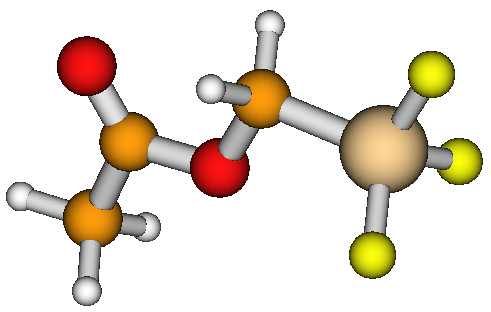
\includegraphics[width=5cm]{acetylmethyltrifluor.png} \label{acetylfluro}}
\subfigure[\ce{Si(OCH3)4}]{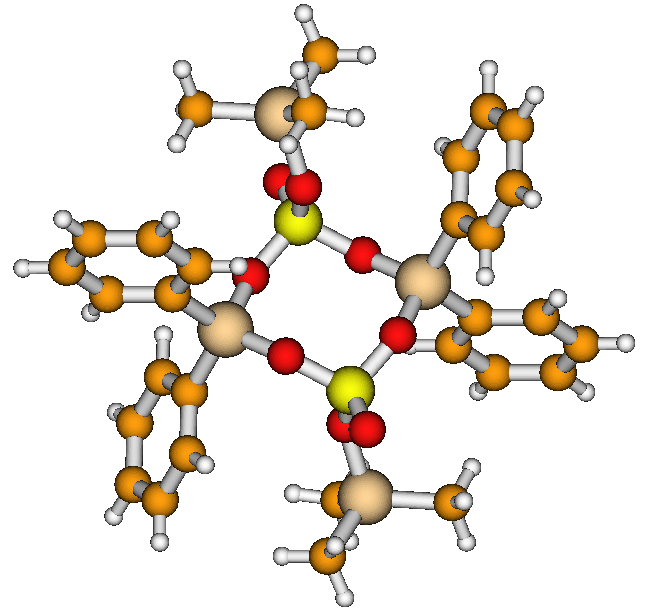
\includegraphics[width=5cm]{rtg_4_kruh_samotne.png}\label{rtg_6}}
\subfigure[\ce{SiCH3(OCH3)5}]{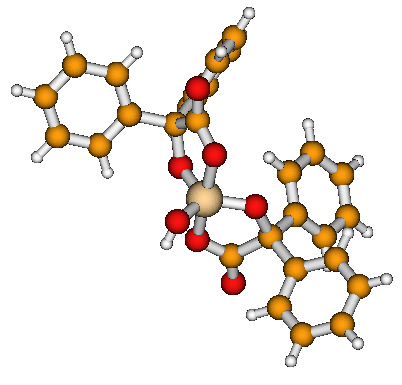
\includegraphics[width=5cm]{rtg_5_koordinace.png}\label{rtg_56}}
\subfigure[\ce{SiCH3(OCH3)5}]{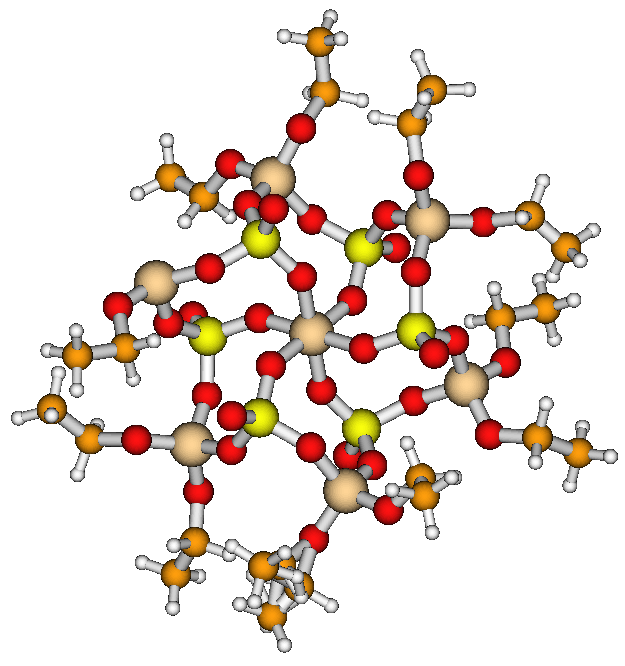
\includegraphics[width=5cm]{rtg_6.png}\label{rtg_55}}
\caption{Přehled reálných struktur.}
\label{prehled_real_structures}
\end{center}
\end{figure}
\subsection{Čtyřkoordinovaný křemík jako reaktant}
Na základě experimentální práce Aleše Stýskalíka jsem se zabývala křemíkem v koordinaci čtyři, který sloužil jako výchozí reaktant pro přípravu silikofosfátových polymerů.

\subsection{Malé modely}
Malé modely podávají podrobnější pohled na charakter vazby Si-C. Obrázky struktur jsou uveden na obrázku \ref{prehled_male_modely}. Pro strukturu \ce{SiCH3(OCH3)5} \ref{si_ch3_och3_5} bylo nutno použit klíčové slovo Opt=CalcFC. Pro sturkturu \ce{Si(OCH3)6} \ref{si_och3_6} byl použit parametr SCF=Vshift. Pro NBO analýzu byly brány HOMO orbitaly.
Přehled výsledků z analýzy NBO je uveden v tabulce \ref{nbo_small}.
\begin{figure}
\begin{center}
\subfigure[\ce{SiCH3(OCH3)3}]{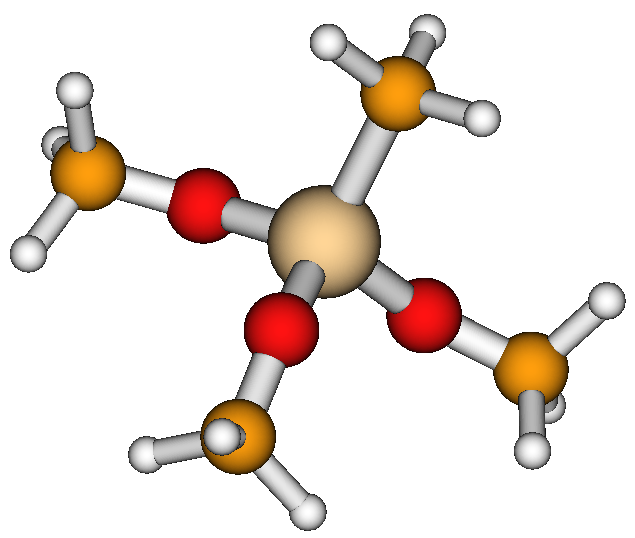
\includegraphics[width=5cm]{si_ch3_och3.png} \label{si_ch3_och3}}
\subfigure[\ce{Si(OCH3)4}]{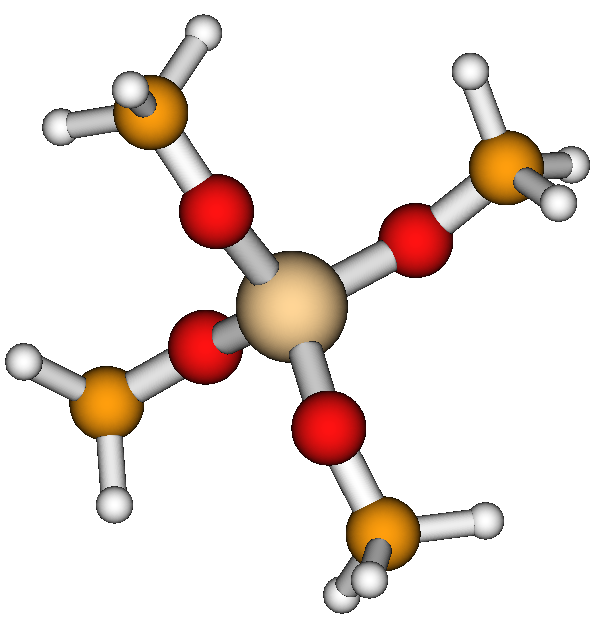
\includegraphics[width=5cm]{si_och3_4.png}\label{si_och3_4}}
\subfigure[\ce{SiCH3(OCH3)5}]{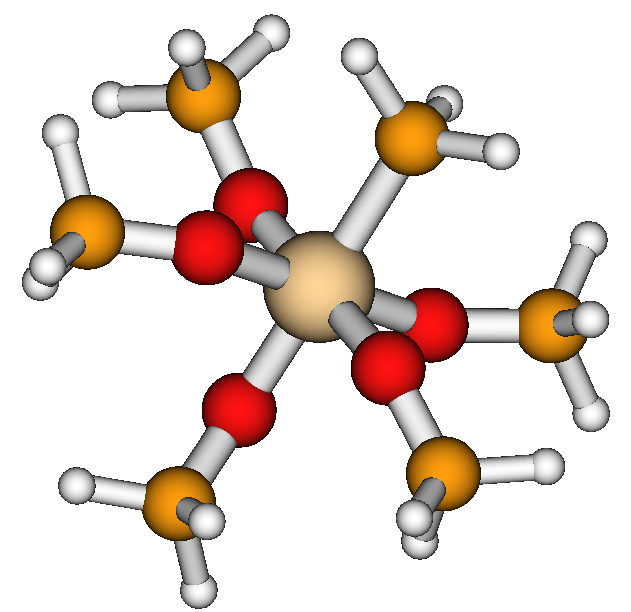
\includegraphics[width=5cm]{si_ch3_och3_5.png}\label{si_ch3_och3_5}}
\subfigure[\ce{Si(OCH3)6}]{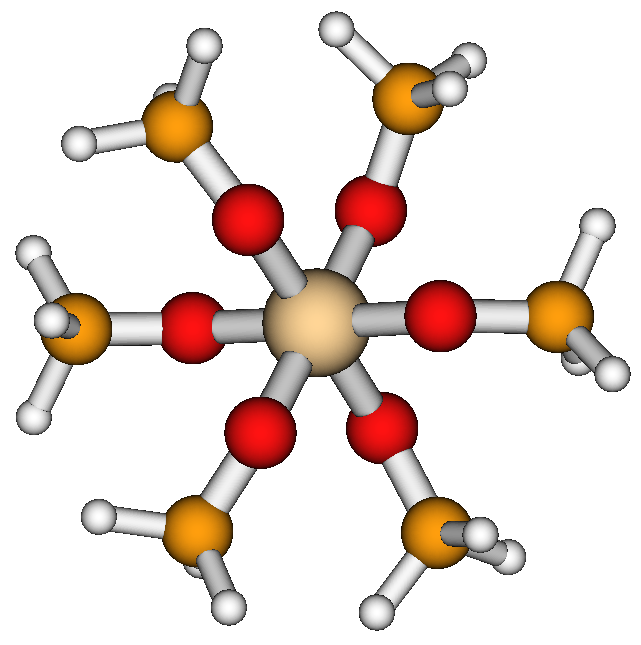
\includegraphics[width=5cm]{si_och3_6.png}\label{si_och3_6}}
\subfigure[\ce{SiCl4}]{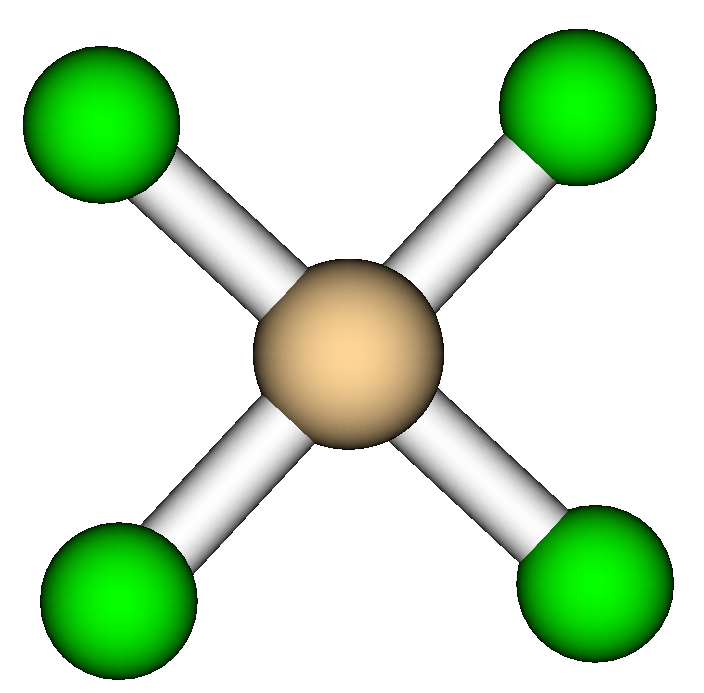
\includegraphics[width=3cm]{si_cl4.png}\label{si_cl4}}
\caption{Přehled malých struktur.}
\label{prehled_male_modely}

\end{center}
\end{figure}
\begin{table}[htbp]
\caption{Výsledky NBO pro malé modely}
\begin{center}
\begin{tabular}{|l|l|l|r|r|r|r|r|r|}
\hline
 &  & vazby & \multicolumn{1}{l|}{Obs.čislo} & \multicolumn{1}{l|}{Si} & \multicolumn{1}{l|}{X} & \multicolumn{1}{l|}{Si(s)} & \multicolumn{1}{l|}{Si(p)} & \multicolumn{1}{l|}{Si(d)} \\ \hline
A & Si-O & 1-2  & 0,066 & 88,3\% & 11,7\% & 23,9\% & 51,9\% & 24,2\% \\ \hline
 &  & 1-3 & 0,111 & 86,5\% & 13,5\% & 23,2\% & 73,3\% & 3,5\% \\ \hline
 &  & 1-3 & 0,092 & 97,1\% & 2,9\% & 0,2\% & 56,7\% & 43,3\% \\ \hline
 &  & 1-4 & 0,065 & 88,5\% & 11,5\% & 23,6\% & 50,2\% & 26,2\% \\ \hline
 & Si-C & 1-17 & 0,073 & 75,5\% & 24,5\% & 29,3\% & 68,9\% & 1,8\% \\ \hline
B & Si-O &1-2,3,4,5  & 0,104 & 86,1\% & 13,9\% & 25,0\% & 71,4\% & 3,6\% \\ \hline
C & Si-O & 1-2  & 0,100 & 92,1\% & 7,9\% & 16,0\% & 50,0\% & 33,9\% \\ \hline
 &  & 1-3 & 0,104 & 91,9\% & 8,1\% & 15,0\% & 50,6\% & 34,4\% \\ \hline
 &  & 1-4 & 0,096 & 91,9\% & 8,1\% & 16,5\% & 50,4\% & 33,1\% \\ \hline
 &  & 1-5 & 0,095 & 91,9\% & 8,1\% & 16,4\% & 50,6\% & 33,0\% \\ \hline
 &  & 1-6 & 0,103 & 92,1\% & 7,9\% & 16,1\% & 50,1\% & 33,8\% \\ \hline
 D& Si-C & 1-27 & 0,068 & 84,6\% & 15,4\% & 22,8\% & 51,2\% & 26,1\% \\ \hline
E & Si-O &Si-2,3,4,5,6,7  & 0,098 & 91,8\% & 8,2\% & 16,7\% & 50,0\% & 33,3\% \\ \hline
F & Si-Cl & 1-2  & 0,125 & 77,9\% & 22,1\% & 24,9\% & 50,0\% & 25,1\% \\ \hline
 &  & 1-3 & 0,125 & 77,9\% & 22,1\% & 24,9\% & 50,0\% & 25,1\% \\ \hline
 &  & 1-4 & 0,125 & 77,9\% & 22,1\% & 24,9\% & 50,0\% & 25,1\% \\ \hline
 &  & 1-5 & 0,125 & 77,9\% & 22,1\% & 24,9\% & 50,0\% & 25,1\% \\ \hline
\end{tabular}
\end{center}
\label{nbo_small}
\end{table}

\subsection{Středně velké modely}
Tato část se věňuje nejmenším možným modelům, které již tvoří uvnitř svých struktur cyklus. Jako referenční molekula byl použita \ce{(acetylmethoxyl)trifluorsilan} z článku \ref{Chipanina2011}. Strutktura \ce{(acetylmethoxyl)trifluorsilan} slouží jako model křemíku v koordinaci čtyři, který má ve svém okolí vysoce elektronegativní atomy. To podporuje teoretické předpoklady o hypervalenci křemíku, pokud má ve svém okolí silně elektronegativní prvek.
\begin{figure}
\begin{center}
\subfigure[(acetylmethoxyl)trifluorsilan]{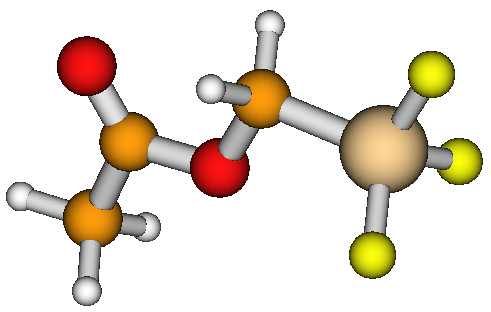
\includegraphics[width=5.5cm]{acetylmethyltrifluor.png} \label{obr_h4sio4_MO_s1_1}}
\subfigure[\ce{SiCH3(PO4(CH3)2)(Si2P2O9(CH3)4)}]{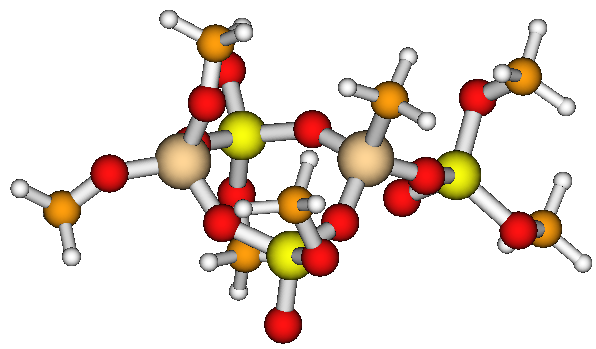
\includegraphics[width=6cm]{si_model_methyl.png}\label{obr_h4sio4_MO_s1_20}}
\subfigure[\ce{Si(Si2P2O9(CH3)4)2}]{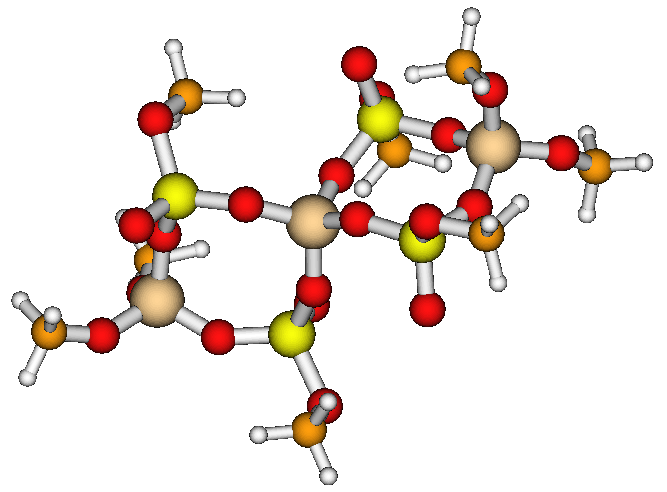
\includegraphics[width=5cm]{si_model_orezany.png}\label{obr_h4sio4_MO_s1_24}}
\caption{Přehled středně velkých modelů}
\label{prehled_middle}
\end{center}
\end{figure}
Pro zvolené sloučeniny byla provedena analýza kanonických orbitalů, výsledky jsou uvedeny v tabulce.
\begin{table}[htbp]
\caption{Výsledky NBO pro středně velké modely}
\begin{center}
\begin{tabular}{|l|l|r|r|r|r|r|r|}
\hline
 & Vazby & \multicolumn{1}{l|}{Obs.číslo} & \multicolumn{1}{l|}{Si} & \multicolumn{1}{l|}{X} & \multicolumn{1}{l|}{Si(s)} & \multicolumn{1}{l|}{Si(p)} & \multicolumn{1}{l|}{Si(d)} \\ \hline
A  & Si-F & 0,107 & 87,1\% & 12,9\% & 22,5\% & 75,6\% & 2,0\% \\ \hline
 & Si-F & 0,107 & 87,1\% & 13,0\% & 22,7\% & 75,4\% & 1,9\% \\ \hline
 & Si-F & 0,107 & 87,1\% & 13,0\% & 22,7\% & 75,4\% & 1,9\% \\ \hline
 & Si-C & 0,079 & 74,3\% & 25,7\% & 32,2\% & 65,8\% & 2,0\% \\ \hline
 & Si-O & 0,087 & 87,5\% & 12,5\% & 23,8\% & 73,1\% & 3,1\% \\ \hline
B & Si-O & 0,093 & 87,3\% & 12,7\% & 23,0\% & 73,5\% & 3,6\% \\ \hline
 & Si-O & 0,094 & 87,5\% & 12,5\% & 22,6\% & 73,9\% & 3,4\% \\ \hline
 & Si-C & 0,065 & 74,1\% & 25,9\% & 30,7\% & 67,7\% & 1,6\% \\ \hline
C & Si-O & 0,086 & 87,1\% & 12,9\% & 25,7\% & 71,1\% & 3,3\% \\ \hline
 & Si-O & 0,104 & 87,4\% & 12,6\% & 23,9\% & 72,5\% & 3,6\% \\ \hline
 & Si-O & 0,098 & 87,2\% & 12,8\% & 24,6\% & 71,9\% & 3,5\% \\ \hline
 & Si-O & 0,092 & 86,8\% & 13,2\% & 25,8\% & 70,8\% & 3,4\% \\ \hline
\end{tabular}
\end{center}
\label{nbo_middle}
\end{table}

\subsection{Velké modely}
\begin{figure}
\begin{center}
\caption{Přehled velkých modelů}
\subfigure[(acetylmethoxyl)trifluorsilan]{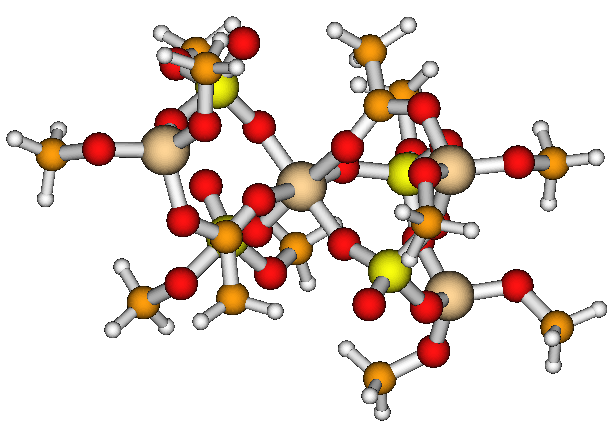
\includegraphics[width=5cm]{struktura_cis.png} \label{obr_h4sio4_MO_s1_1}}
\subfigure[]{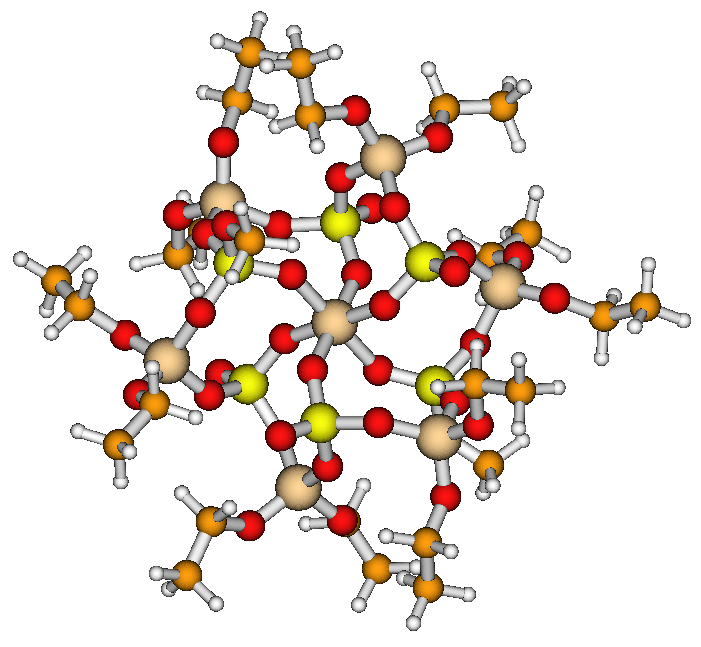
\includegraphics[width=5cm]{srtuktura_bez_naboje.png}\label{obr_h4sio4_MO_s1_20}}
\subfigure[]{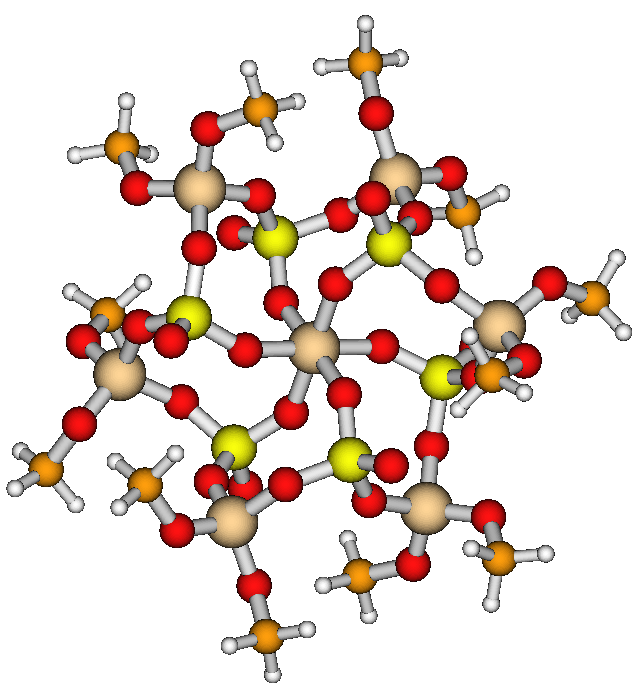
\includegraphics[width=5cm]{struktura_puvodni.png}\label{obr_h4sio4_MO_s1_24}}
\subfigure[]{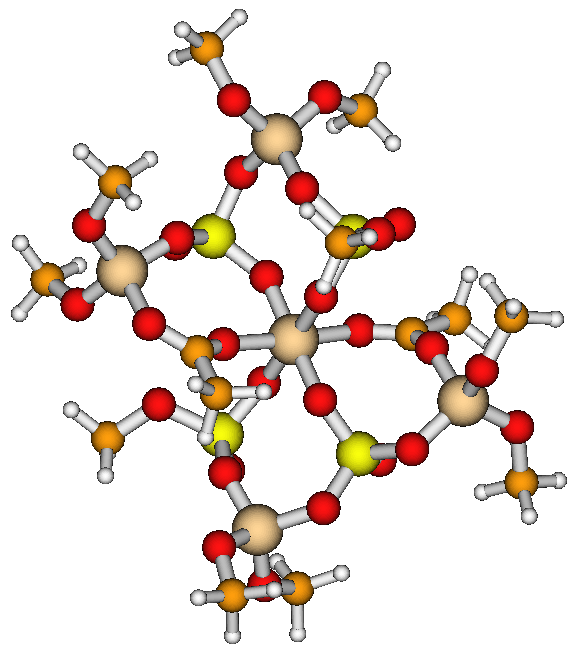
\includegraphics[width=5cm]{struktura_trans.png}\label{obr_h4sio4_MO_s1_24}}
\label{prehled_large}
\end{center}
\end{figure}
\begin{table}[htbp]
\caption{Výsledky NBO pro velké modely}
\begin{center}
\begin{tabular}{|l|l|l|r|r|r|r|r|r|}
\hline
 &  &  & \multicolumn{1}{l|}{Obs.čislo} & \multicolumn{1}{l|}{Si} & \multicolumn{1}{l|}{X} & \multicolumn{1}{l|}{Si(s)} & \multicolumn{1}{l|}{Si(p)} & \multicolumn{1}{l|}{Si(d)} \\ \hline
A & Si-O & 1-2  & 0,089 & 91,33 \% & 8,67 \% & 17,15 \% & 49,89 \% & 32,96 \% \\ \hline
 &  & 1-3  & 0,105 & 92,66 \% & 7,34 \% & 16,06 \% & 50,23 \% & 33,72 \% \\ \hline
 &  & 1-4  & 0,088 & 91,24 \% & 8,76 \% & 17,21 \% & 50,07 \% & 32,72 \% \\ \hline
 &  & 1-5  & 0,089 & 91,48 \% & 8,52 \% & 16,70 \% & 50,16 \% & 33,13 \% \\ \hline
 &  & 1-6 & 0,104 & 92,53 \% & 7,47 \% & 16,29 \% & 49,80 \% & 33,91 \% \\ \hline
 &  & 1-7 & 0,088 & 91,29 \% & 8,71 \% & 16,98 \% & 49,95 \% & 33,08 \% \\ \hline
B & Si-O & 1-3  & 0,175 & 89,18 \% & 10,82 \% & 31,84 \% & 64,07 \% & 4,08 \% \\ \hline
 &  & 1-4  & 0,171 & 88,78 \% & 11,22 \% & 33,01 \% & 63,00 \% & 4,00 \% \\ \hline
 &  & 1-5  & 0,132 & 88,88 \% & 11,12 \% & 16,88 \% & 79,32 \% & 3,80 \% \\ \hline
 &  & 1-7 & 0,127 & 88,94 \% & 11,06 \% & 16,73 \% & 79,55 \% & 3,72 \% \\ \hline
C & Si-O & 1-2  & 0,106 & 90,65 \% & 9,35 \% & 22,30 \% & 52,16 \% & 25,54 \% \\ \hline
 &  & 1-4  & 0,113 & 90,69 \% & 9,31 \% & 22,02 \% & 51,83 \% & 26,15 \% \\ \hline
 &  & 1-5  & 0,161 & 90,48 \% & 9,52 \% & 9,91 \% & 86,47 \% & 3,62 \% \\ \hline
 &  & 1-6 & 0,111 & 90,57 \% & 9,43 \% & 21,86 \% & 52,57 \% & 25,57 \% \\ \hline
 &  & 1-7 & 0,104 & 90,19 \% & 9,43 \% & 23,30 \% & 51,81 \% & 24,89 \% \\ \hline
D & Si-O & 1-2  & 0,092 & 91,57 \% & 8,43 \% & 16,92 \% & 50,05 \% & 33,03 \% \\ \hline
 &  & 1-3  & 0,094 & 91,82 \% & 8,18 \% & 16,49 \% & 50,05 \% & 33,46 \% \\ \hline
 &  & 1-4  & 0,092 & 91,67 \% & 8,33 \% & 16,73 \% & 49,90 \% & 33,37 \% \\ \hline
 &  & 1-5  & 0,093 & 91,74 \% & 8,26 \% & 16,54 \% & 49,96 \% & 33,50 \% \\ \hline
 &  & 1-6 & 0,093 & 91,73 \% & 8,27 \% & 16,72 \% & 49,96 \% & 33,32 \% \\ \hline
 &  & 1-7 & 0,093 & 91,75 \% & 8,25 \% & 16,59 \% & 50,11 \% & 33,30 \% \\ \hline
E & Si-O & 1-2  & 0,091 & 91,63 \% & 8,37 \% & 17,13 \% & 50,11 \% & 32,76 \% \\ \hline
 &  & 1-3  & 0,115 & 89,41 \% & 10,59 \% & 20,87 \% & 63,97 \% & 15,16 \% \\ \hline
 &  & 1-4  & 0,085 & 91,53 \% & 8,47 \% & 17,31 \% & 50,82 \% & 31,88 \% \\ \hline
 &  & 1-5  & 0,113 & 90,01 \% & 9,99 \% & 20,02 \% & 62,64 \% & 17,34 \% \\ \hline
 &  & 1-6 & 0,093 & 86,99 \% & 13,01 \% & 24,67 \% & 65,85 \% & 9,48 \% \\ \hline
\end{tabular}
\end{center}
\label{nbo_large}
\end{table}



\section{Vazby}

\section{Spektroskopi}












\chapter{Závěr}


{\csname captions\languagename\endcsname %% Temporarily override
%% the BibLaTeX localization with the original babel definitions.
\makeatletter %% Use the correct localization of the quotations.
  \thesis@selectLocale{\thesis@locale}\makeatother
\printbibliography[heading=bibintoc]} %% Print the bibliography.
\appendix %% Start the appendices.




\end{document}
